\documentclass[11pt, aspectratio=169, compress]{beamer}
\usetheme[progressbar=frame title, numbering=fraction]{metropolis}      % Use metropolis theme 
\setbeamertemplate{section in toc}[sections numbered]
\setbeamertemplate{subsection in toc}[subsections numbered]
\useoutertheme[subsection=false]{miniframes}
\setbeamercolor{section in head/foot}{fg=white, bg=mDarkTeal}
\setbeamercolor{background canvas}{bg=white}
\setbeamerfont{section in head/foot}{series=\bfseries}

\usefonttheme[onlymath]{serif}
\usepackage{amsmath}
\usepackage{remreset}
\usepackage{ragged2e}
\usepackage{booktabs}
\usepackage{makecell}
\usepackage{float}
\usepackage{subfig}
\usepackage{tikz}
\usetikzlibrary{positioning,calc,trees}
\usepackage[flushleft]{threeparttable}	% 3 part table 
\usepackage[justification=centering]{caption}
\captionsetup{skip=0pt}
\graphicspath{{./fig/}}

\makeatletter
\let\beamer@writeslidentry@miniframeson=\beamer@writeslidentry
\def\beamer@writeslidentry@miniframesoff{%
	\expandafter\beamer@ifempty\expandafter{\beamer@framestartpage}{}% does not happen normally
	{%else
		% removed \addtocontents commands
		\clearpage\beamer@notesactions%
	}
}
\newcommand*{\miniframeson}{\let\beamer@writeslidentry=\beamer@writeslidentry@miniframeson}
\newcommand*{\miniframesoff}{\let\beamer@writeslidentry=\beamer@writeslidentry@miniframesoff}
\beamer@compresstrue
\makeatother

%==============================================================
% Title Page
%==============================================================
%Information to be included in the title page:
\title{Manejo y Limpieza de Datos}
\author{Rony Rodriguez-Ramírez} 
\institute{LAMBDA}
\titlegraphic{\hfill
\includegraphics[height=1.5cm]{dime}}
\date{\today}
%==============================================================
\begin{document}
%------------------------------------------------	
\begin{frame}[plain]
	\maketitle 
\end{frame}
%------------------------------------------------
\section{Manejo de Datos}
%-----------------------------------------------
\subsection{Manejo de Datos}
%-----------------------------------------------
\begin{frame}{Pensemos en replicabilidad}
	El fin de esta sesión es asegurar que nuestras investigación sea reproducible. 
	\begin{itemize}
		\item Publicar un artículo por sí solo ya no es suficiente:
		\begin{itemize}
			\item Al igual que las tablas y las figuras, el código ahora es un resultado igualmente importante para compartir. En este contexto, publicar código no tiene sentido si es:
			\begin{enumerate}
				\item no reproducible. 
				\item nadie puede entender como se corre.
			\end{enumerate}
			\item Para que el código sea útil, requiere transparencia, responsabilidad y un flujo de trabajo fácil de entender.
			\item Básicamente, el código debe ser organizado y legible. 
		\end{itemize}
	\end{itemize}
\end{frame}
%-----------------------------------------------
\begin{frame}{Esto es mucho más fácil decirlo que hacerlo}
	\begin{itemize}
		\item En DIME, tenemos grandes equipos que colaboran en los mismos códigos y conjuntos de datos. 
		\item Los proyectos grandes se vuelven fácilmente complejos ya que tienen múltiples rondas / fuentes de datos que deben organizarse.
		\item La estandarización de la organización de documentos y códigos previene errores y reduce el costo de la transición entre proyectos y equipos.
	\end{itemize}
\end{frame}
%-----------------------------------------------
\begin{frame}{¿A qué nos referimos con gestión de datos?}
	En esta sesión entenderemos e implementaremos las mejores prácticas para gestionar el trabajo de datos a través de:
	\begin{itemize}
		\item Configurar una buena estructura de carpetas
		\item Crear un script maestro que ejecute todo el código
		\item Establecer un sistema de control de versiones
	\end{itemize}
	Cuando los contenidos de esta sesión se aplican a un proyecto, cualquier persona con acceso completo a sus archivos y carpetas  podrá replicar la investigación y comprender la estructura del trabajo de datos.
\end{frame}
%-----------------------------------------------
\section{Estructura de las carpetas}
\subsection{Estructura de las carpetas}
%-----------------------------------------------
\begin{frame}[t]{¿Por qué nos debería importar la estructura de nuestros folderes?}
	\begin{itemize}
		\item La carpeta de su proyecto probablemente tenga muchas subcarpetas para literatura, presentaciones, notas conceptuales y otros documentos.
		\item En esta sesión, nos centraremos en las carpetas relacionadas con el trabajo de datos. Llamaremos al conjunto de carpetas relacionadas con datos la carpeta DataWork.
	\end{itemize}
\end{frame}
%-----------------------------------------------
\begin{frame}[t]{¿Por qué nos debería importar la estructura de nuestros folderes?}
	\begin{itemize}
		\item El paquete \texttt{ietoolkit} Stata ofrece un comando llamado \texttt{iefolder} que ayuda a configurar la estructura de carpetas y sus interacciones con los archivos de código. 
		\item \texttt{Iefolder} proporciona una plantilla para la estructura de carpetas para un proyecto DIME típico utilizando datos primarios.
		\item No entraremos en detalles sobre cómo usar el comando \texttt{iefolder} aquí, sino que nos centraremos en los principios detrás de él.
		\item Para obtener documentación y detalles sobre cómo usar el comando, escriba \texttt{help iefolder} en Stata.
	\end{itemize}
\end{frame}
%-----------------------------------------------
\begin{frame}[t]{¿Por qué nos debería importar la estructura de nuestros folderes?}
	\begin{itemize}
		\item La motivación detrás de iefolder es crear una estructura estandarizada que sea fácil de navegar para los miembros del equipo.
		\item Los diferentes proyectos pueden tener necesidades específicas, pero las plantillas utilizadas en iefolder son un buen punto de partida para pensar en la estructura de carpetas de cualquier proyecto.
		\item Sin embargo, sea cual sea la estructura que esté utilizando, aplicarla a todos sus proyectos hará que sea más fácil moverse entre proyectos.
	\end{itemize}
\end{frame}
%-----------------------------------------------
\begin{frame}[t]{DataWork Folder: Visión General}
	\begin{columns}
		\begin{column}{0.5\textwidth}
		   \begin{itemize}
			   \item Así es como se ve la carpeta \texttt{DataWork} creada por \texttt{iefolder}:
		   \end{itemize}
		\end{column}
		\begin{column}{0.5\textwidth} 
			\tikzstyle{every node}=[draw=black,thick,anchor=west]
			\tikzstyle{selected}=[draw=red,fill=red!30]
			\tikzstyle{optional}=[dashed,fill=gray!50]
			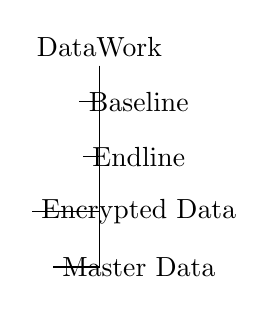
\begin{tikzpicture}[%
				grow via three points={one child at (0.5,-0.7) and
				two children at (0.5,-0.7) and (0.5,-1.4)},
				edge from parent path={(\tikzparentnode.south) |- (\tikzchildnode.west)}]
				\node {DataWork}
				  child { node {Baseline}}		  
				  child { node {Endline}}
				  child { node {Encrypted Data}}
				  child { node {Master Data}};
			  \end{tikzpicture}
		\end{column}
	\end{columns}
\end{frame}
%-----------------------------------------------
\begin{frame}[t]{DataWork Folder: Visión General}
	\begin{columns}
		\begin{column}{0.5\textwidth}
		   \begin{itemize}
			   \item La carpeta de línea de base (baseline) almacenará todos los datos de línea de base, así como los archivos do y las salidas que se refieren exclusivamente a esta ronda de recopilación de datos.
		   \end{itemize}
		\end{column}
		\begin{column}{0.5\textwidth} 
			\tikzstyle{every node}=[draw=black,thick,anchor=west]
			\tikzstyle{selected}=[draw=red,fill=red!30]
			\tikzstyle{optional}=[dashed,fill=gray!50]
			\begin{tikzpicture}[%
				grow via three points={one child at (0.5,-0.7) and
				two children at (0.5,-0.7) and (0.5,-1.4)},
				edge from parent path={(\tikzparentnode.south) |- (\tikzchildnode.west)}]
				\node {DataWork}
				  child { node [selected] {Baseline}
					child { node {\small DataSets}}
					child { node {\small Dofiles}}
					child { node {\small Outputs}}
					child { node {\small Documentation}}
					child { node {\small Questionnaire}}
				  }		
				  child [missing] {}				
				  child [missing] {}				
				  child [missing] {}	
				  child [missing] {}				
				  child [missing] {}		  
				  child { node {Endline}}
				  child { node {Encrypted Data}}
				  child { node {Master Data}};
			  \end{tikzpicture}
		\end{column}
	\end{columns}
\end{frame}
%-----------------------------------------------
\begin{frame}[t]{DataWork Folder: Visión General}
	\begin{columns}
		\begin{column}{0.5\textwidth}
		   \begin{itemize}
			   \item La carpeta de la línea final almacenará todos los datos de la línea final, así como el código y las salidas que se refieren exclusivamente a esta ronda de recopilación de datos. 
			   \item Tenga en cuenta que su estructura es exactamente la misma que la estructura de la carpeta de línea de base.
		   \end{itemize}
		\end{column}
		\begin{column}{0.5\textwidth} 
			\tikzstyle{every node}=[draw=black,thick,anchor=west]
			\tikzstyle{selected}=[draw=red,fill=red!30]
			\tikzstyle{optional}=[dashed,fill=gray!50]
			\begin{tikzpicture}[%
				grow via three points={one child at (0.5,-0.7) and
				two children at (0.5,-0.7) and (0.5,-1.4)},
				edge from parent path={(\tikzparentnode.south) |- (\tikzchildnode.west)}]
				\node {DataWork}
				child { node {Baseline}}				  
				child { node [selected] {Endline}
				child { node {\small DataSets}}
				child { node {\small Dofiles}}
				child { node {\small Outputs}}
				child { node {\small Documentation}}
				child { node {\small Questionnaire}}
				}
				child [missing] {}				
				child [missing] {}				
				child [missing] {}	
				child [missing] {}				
				child [missing] {}
				child { node {Encrypted Data}}
				child { node {Master Data}};
				\end{tikzpicture}
		\end{column}
	\end{columns}
\end{frame}
%-----------------------------------------------
\begin{frame}{DataWork: Round Folders}
	\begin{itemize}
		\item Si bien una ronda de recopilación de datos solo puede parecer aplicable a los datos primarios, puede pensar en una ``ronda'' como una fuente de recopilación de datos.
		\item Otra forma de decirlo es pensar en una ``ronda'' como un conjunto de datos que se procesarán con el mismo código
	\end{itemize}
\end{frame}
%-----------------------------------------------
\begin{frame}{DataWork: Round Folders}
	\begin{itemize}
		\item Un ejemplo de esto podría ser una recopilación de datos primarios que incluye dos niveles de observación (hogar y comunidad, estudiante y escuela, paciente y médico, etc.): cada nivel probablemente tendrá su propio cuestionario y se limpiará por separado.
		\item Por lo tanto, creará diferentes carpetas, como \texttt{HouseholdBaseline} y \texttt{CommunityBaseline}.
		\item Otro ejemplo es cuando el mismo cuestionario se aplica dos veces, pero los nombres de las variables y las etiquetas de valor son ligeramente diferentes. Entonces también necesitarás dos carpetas separadas.
	\end{itemize}
\end{frame}
%-----------------------------------------------
\begin{frame}[t]{DataWork: Carpeta encryptada (datos cifrados)}
	\begin{columns}
		\begin{column}{0.5\textwidth}
		   \begin{itemize}
			   \item La carpeta de datos cifrados contendrá todos los datos de identificación personal para cada ronda de recopilación de datos, y una carpeta con claves maestras de identificación que vincula cada identificación no identificada a las observaciones identificadas.   
			  \item Como su nombre indica, esta carpeta debe estar encriptada.
		   \end{itemize}
		\end{column}
		\begin{column}{0.5\textwidth} 
			\tikzstyle{every node}=[draw=black,thick,anchor=west]
			\tikzstyle{selected}=[draw=red,fill=red!30]
			\tikzstyle{optional}=[dashed,fill=gray!50]
			\begin{tikzpicture}[%
				grow via three points={one child at (0.5,-0.7) and
				two children at (0.5,-0.7) and (0.5,-1.4)},
				edge from parent path={(\tikzparentnode.south) |- (\tikzchildnode.west)}]
				\node {DataWork}
				child { node {Baseline}}				  
				child { node {Endline}}
				child { node [selected] {Encrypted Data}
				child {node {IDMasterKey}}
				child {node {Baseline}}
				child {node {Endline}}
				}
				child [missing] {}	
				child [missing] {}				
				child [missing] {}
				child { node {Master Data}};
				\end{tikzpicture}
		\end{column}
	\end{columns}
\end{frame}
%-----------------------------------------------
\begin{frame}[t]{DataWork: Master Data}
	\begin{columns}
		\begin{column}{0.5\textwidth}
		   \begin{itemize}
			   \item La carpeta de datos maestros (master data) almacenará los conjuntos de datos maestros para cada unidad de observación en su proyecto.
		   \end{itemize}
		\end{column}
		\begin{column}{0.5\textwidth} 
			\tikzstyle{every node}=[draw=black,thick,anchor=west]
			\tikzstyle{selected}=[draw=red,fill=red!30]
			\tikzstyle{optional}=[dashed,fill=gray!50]
			\begin{tikzpicture}[%
				grow via three points={one child at (0.5,-0.7) and
				two children at (0.5,-0.7) and (0.5,-1.4)},
				edge from parent path={(\tikzparentnode.south) |- (\tikzchildnode.west)}]
				\node {DataWork}
				child { node {Baseline}}				  
				child { node {Endline}}
				child { node {Encrypted Data}}
				child { node [selected] {Master Data}};
				\end{tikzpicture}
		\end{column}
	\end{columns}
\end{frame}
%-----------------------------------------------
\begin{frame}{¿Qué es el master data?}
	\begin{itemize}
		\item Una lista completa o lista completa de todas las observaciones potenciales que uno puede encontrar durante el curso de un proyecto.
		\item Forma una documentación exhaustiva de las acciones tomadas para cada unidad de observación en el alcance del proyecto.
		\item Un ejemplo: un conjunto de datos maestros del hogar incluirá:
		\begin{itemize}
			\item hogares enumerados en el censo.
			\item hogares muestreados para las encuestas.
			\item hogares incluidos en el monitoreo (incluso si no son parte del proyecto).
			\item hogares incluidos en el análisis.
			\item una identificación única para cada uno de estos hogares.
		\end{itemize}
	\end{itemize}
\end{frame}
%-----------------------------------------------
\section{Usando la carpeta de DataWork}
\subsection{Usando la carpeta de DataWork}
%-----------------------------------------------
\begin{frame}{Base de datos}
	\begin{itemize}
		\item Todas las bases de datos a ocupar deben de estar de-idenficadas.
	\end{itemize}
	\tikzstyle{every node}=[draw=black,thick,anchor=west]
	\tikzstyle{selected}=[draw=red,fill=red!30]
	\tikzstyle{optional}=[dashed,fill=gray!50]
	\begin{center}
		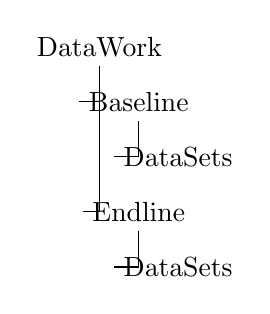
\begin{tikzpicture}[%
			grow via three points={one child at (0.5,-0.7) and
			two children at (0.5,-0.7) and (0.5,-1.4)},
			edge from parent path={(\tikzparentnode.south) |- (\tikzchildnode.west)}]
			\node {DataWork}
			child { node {Baseline}
			child {node {DataSets}}}	
			child [missing] {}			  
			child { node {Endline}
			child {node {DataSets}}};
		\end{tikzpicture}	
	\end{center}
\end{frame}
%-----------------------------------------------
\begin{frame}{Base de datos}
	\begin{itemize}
		\item Las secuencias de comandos en cada carpeta cargarán datos de la carpeta de bases de datos de esa ronda y almacenarán cualquier salida en la carpeta de salidas de la ronda.
	\end{itemize}
	\begin{center}
		\tikzstyle{every node}=[draw=black,thick,anchor=west]
		\tikzstyle{selected}=[draw=red,fill=red!30]
		\tikzstyle{optional}=[draw=gray,fill=gray!20]
		\begin{tikzpicture}[%
			grow via three points={one child at (0.5,-0.7) and
			two children at (0.5,-0.7) and (0.5,-1.4)},
			edge from parent path={(\tikzparentnode.south) |- (\tikzchildnode.west)}]
			\node {DataWork}
			child {node [selected] {Baseline}
			child {node [selected] {\footnotesize Datasets}}
			child {node [selected] {\footnotesize Dofiles}}
			child {node [selected] {\footnotesize Outputs}}
			child {node [optional] {\footnotesize Documentation}}
			child {node [optional] {\footnotesize Questionnaire}}}; 
		\end{tikzpicture}
	\end{center}	
\end{frame}
%-----------------------------------------------
\section{Master Script}
\subsection{Master Script}
%-----------------------------------------------
\begin{frame}{¿Por qué es necesario un script maestro?}
	\begin{itemize}
		\item Como habrás notado, mencionamos la creación de muchos scripts de código en las diapositivas anteriores.
		\item Un gran proyecto puede volverse muy complejo, y las secuencias de comandos deben ejecutarse en un cierto orden para crear la salida correcta.
	\end{itemize}
\end{frame}
%-----------------------------------------------
\begin{frame}{¿Por qué es necesario un script maestro?}
	\begin{itemize}
		\item Eso podría significar que necesitaría escribir una secuencia de comandos extremadamente larga o un documento diferente con instrucciones sobre en qué orden ejecutar todas las secuencias de comandos.
		\item Sin embargo, puede crear un script que ejecute otros scripts.
		\item Esto facilita que cualquiera que reproduzca su código lo haga con facilidad.
	\end{itemize}
\end{frame}
%-----------------------------------------------
\begin{frame}{¿Qué es un script maestro?}
	\begin{itemize}
		\item El script maestro es el mapa sobre todo el trabajo de datos en su carpeta de datos
		\item Es la tabla de contenido para las instrucciones que codifica
		\item Debería ser posible seguir todo el trabajo de datos en la carpeta de datos, desde datos sin procesar hasta resultados de análisis, leyendo el script maestro. 
	\end{itemize}
\end{frame}
%-----------------------------------------------
\begin{frame}{Script maestro: permite una colaboración fácil}
	\begin{itemize}
		\item Si compartimos un proyecto a través de DropBox o GitHub, todos los miembros del equipo tienen la misma estructura de carpetas.
		\item Un script maestro permite que varias personas establezcan su propio global en la carpeta del proyecto.
		\item De esta manera, cualquiera que comparta la carpeta del proyecto puede ejecutar fácilmente sus scripts.
	\end{itemize}
\end{frame}
%-----------------------------------------------
\begin{frame}{Script maestro: Connexión entre código y estructura de carpetas}
	\begin{itemize}
		\item El script maestro contiene \texttt{globals} u objetos que hacen referencia a la subcarpeta en la carpeta \texttt{DataWork}, por lo que tiene accesos directos fáciles para ellos.
		\item Cualquier cambio en la estructura de carpetas puede explicarse fácilmente cambiando el global de la carpeta.
	\end{itemize}
\end{frame}
%-----------------------------------------------
\begin{frame}{Script maestro: Connexión entre código y estructura de carpetas}
	\begin{figure}[H]
		\centering
		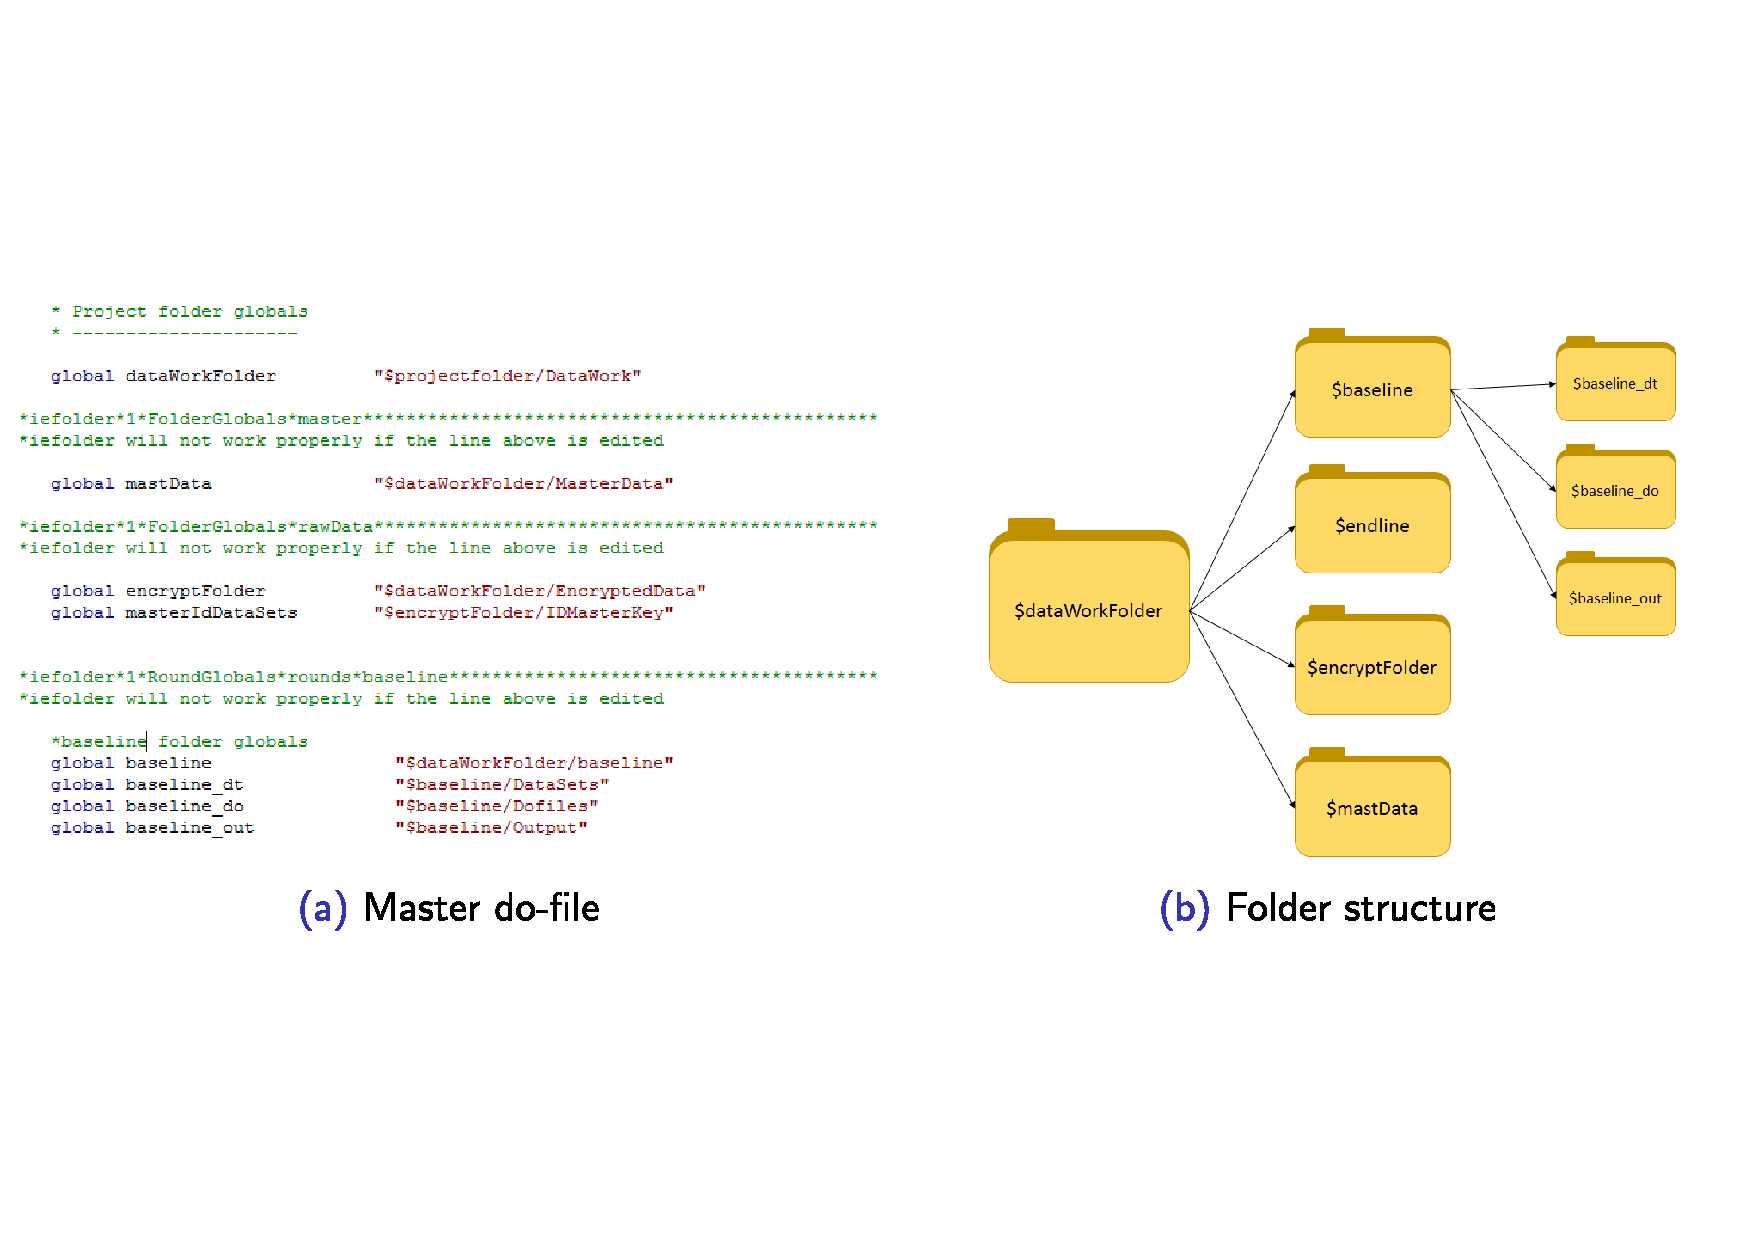
\includegraphics[width=1\textwidth]{code_structure.pdf}
	\end{figure}
\end{frame}
%-----------------------------------------------
\begin{frame}{Script maestro: Permite actualizaciones fáciles}
	\begin{itemize}
		\item Las entradas del usuario y la configuración global deben definirse en el script maestro.
		\item Ejemplos de esto incluyen rutas de carpeta, tasas de conversión, control y variables de resultado, e incluso colores de gráficos
		\item Esto le permite realizar cambios en una sola línea de código a través de un objeto global o cuando quiera aplicar una actualización a todos sus códigos.
		\item Si está utilizando Stata, los globales solo deben definirse en el do file maestro.
	\end{itemize}
\end{frame}
%-----------------------------------------------
\begin{frame}{Script maestro: Permite replicaciones fáciles}
	\begin{itemize}
		\item Cualquiera debería poder seguir y reproducir todo su trabajo desde los datos en bruto a todas las salidas con un clic en este script, después de agregar solo la ruta de la carpeta raíz.
		\item En general, siempre debe ejecutar códigos a través del script maestro Esto evita el flujo de trabajo muy común de ejecutar este script, luego este y finalmente el otro.
		\item También le ayuda a asegurarse de que los cambios que realice en un código no rompan otros códigos.
	\end{itemize}
\end{frame}
%-----------------------------------------------
\begin{frame}{Script maestro: El mapa a todo el trabajo de datos}
	\begin{itemize}
		\item Al leer el script maestro, alguien externo al proyecto debe tener una comprensión general de lo que se está haciendo en cada paso

		\item Si desea ver cómo se creó o creó una tabla o conjunto de datos en particular, leer el script maestro debería ser suficiente para decir qué script mirar.
		
		\item El uso de locales y objetos para crear interruptores para seleccionar qué partes del proyecto ejecutar o no facilitar el uso del código cuando los proyectos son muy largos y complejos.
	\end{itemize}
\end{frame}
%-----------------------------------------------
\begin{frame}{Prácticas recomendadas para rutas de archivos}
	\begin{figure}[H]
		\centering
		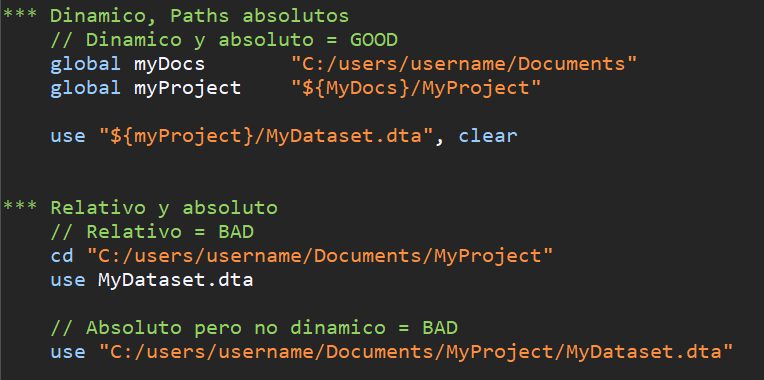
\includegraphics[width=0.8\textwidth]{paths.png}
	\end{figure}	
\end{frame}
%-----------------------------------------------
\end{document}		
